\documentclass[12pt]{article}
\usepackage[a4paper, total={5.5in, 9in}]{geometry}
\usepackage{amsmath}
\usepackage{amsfonts}
\usepackage{graphicx}
\usepackage{pgfplots}
\pgfplotsset{compat=1.18}
\usepackage{enumitem}

\title{College Algebra Worksheet 3.6}
\author{PCL Learning Center}
\date{}

\begin{document}
\maketitle

\begin{center}
    \textit{note: No graphing calculators or electronic devices may be used on this worksheet.}    
\end{center}

\section*{Problem Set 1\\Difficulty level: Normal}
\subsection*{Problem 1}
Find the solutions to the following absolute value equation.
\[4|x-9|+2=7\]

\subsection*{Problem 2}
Find the solutions to the following absolute value equation
\[11|x+3|+9=10\]

\subsection*{Problem 3}
Identify the parent function of \(f(x)=(x+3)^3\).

\subsection*{Problem 4}
Given the following piecewise function, evaluate \(f(4)\).
\[
f(x) = \begin{cases} 
2x + 5 & \text{if } x < 5 \\ 
-2x + 4 & \text{if } x \geq 5 
\end{cases}
\]

\subsection*{Problem 5}
Identify the parent function of the following graph.

    \begin{center}
    \begin{tikzpicture}
    \begin{axis}[
        axis lines=middle,
        width=10cm,
        height=8cm,
        xmin=-6, xmax=6,
        ymin=-1, ymax=6,
    ]
    \addplot[red, thick, domain=-6:6, samples=100] {(x+1)^3+3};
    \end{axis}
    \end{tikzpicture}
    \end{center}

\subsection*{Problem 6}
Evaluate \(f(3)\) given the piecewise function below.
\[
f(x) = \begin{cases} 
7x + 1 & \text{if } x < 3 \\ 
-5x + 5 & \text{if } x \geq 3 
\end{cases}
\] 

\subsection*{Problem 7}
Fill the following open circles to match the piecewise function shown below.
\[
f(x) = 
\begin{cases} 
-x + 1 & \text{if } x < -4 \\ 
\dfrac{x^2}{2} + x - 2 & \text{if } -4 \leq x \leq 2 \\ 
-x + 3 & \text{if } x > 2 
\end{cases}
\]

\begin{figure}[!ht]
    \centering
    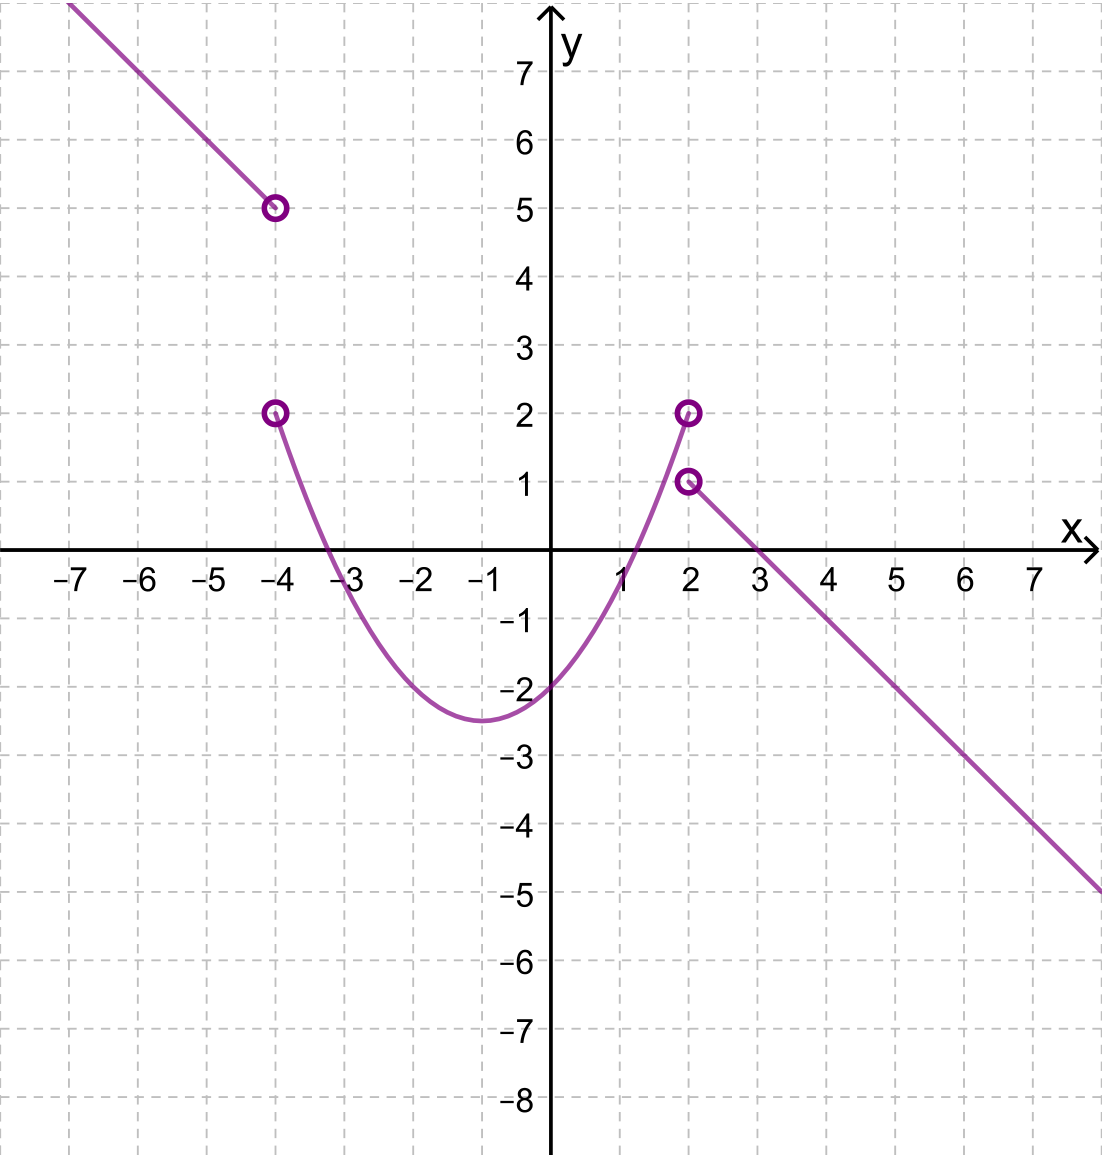
\includegraphics[width=0.4\linewidth]{1.png}
\end{figure}

\subsection*{Problem 8}
Which of the following piecewise functions is represented in the graph below?
\begin{figure}[!ht]
    \centering
    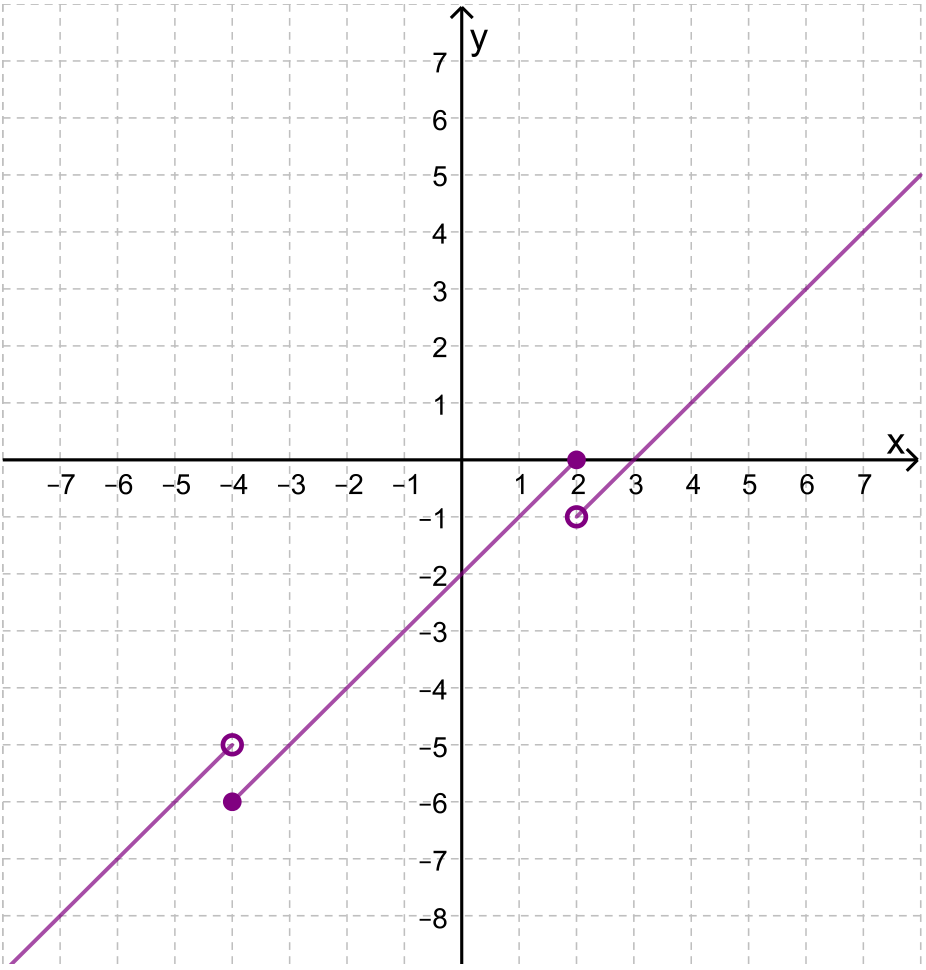
\includegraphics[width=0.5\linewidth]{2.png}
\end{figure}

\begin{enumerate}[label=(\alph*)]
    \item $f(x) = \begin{cases} 
          x - 1 & \text{if } x \leq -4 \\ 
          x - 2 & \text{if } -4 < x < 2 \\ 
          x - 3 & \text{if } x \geq 2 
          \end{cases}$
          
    \item $f(x) = \begin{cases} 
          x - 1 & \text{if } x < -4 \\ 
          x - 2 & \text{if } -4 \leq x < 2 \\ 
          x - 3 & \text{if } x \geq 2 
          \end{cases}$
          
    \item $f(x) = \begin{cases} 
          x - 1 & \text{if } x \leq -4 \\ 
          x - 2 & \text{if } -4 < x \leq 2 \\ 
          x - 3 & \text{if } x > 2 
          \end{cases}$
          
    \item $f(x) = \begin{cases} 
          x - 1 & \text{if } x < -4 \\ 
          x - 2 & \text{if } -4 \leq x \leq 2 \\ 
          x - 3 & \text{if } x > 2 
          \end{cases}$
\end{enumerate}

\subsection*{Problem 9}
Identify the parent function of \(f(x)=(x-4)^2\).

\subsection*{Problem 10}
Given the following piecewise function, evaluate \(f(2)\).
\[
f(x) = 
\begin{cases} 
2x - 2 & \text{if } x < -1 \\ 
x^2 + 3 & \text{if } -1 \leq x < 2 \\ 
-3x & \text{if } x \geq 2 
\end{cases}
\]

\section*{Problem Set 2\\Difficulty level: Hard}
\subsection*{Problem 1}
Describe all numbers \(x\) that are at a distance of 4 from the number 8. Express this set of numbers using absolute value notation.

\subsection*{Problem 2}
Describe all numbers \(x\) that are at a distance of \(\dfrac{1}{2}\) from the number \(-4\). Express this set of numbers using absolute value notation.

\subsection*{Problem 3}
Find the \(x\)- and \(y\)-intercepts of the following absolute value function.
\[f(x)=|-2x+1|-13\]

\newpage
\section*{Solutions to the Set 1}
\subsection*{Problem 1}
\(x=\dfrac{31}{4}\) and \(x=\dfrac{41}{4}\)
\subsection*{Problem 2}
\(x=\dfrac{-34}{11}\) and \(x=\dfrac{-32}{11}\)
\subsection*{Problem 3}
\(x^3\)
\subsection*{Problem 4}
13
\subsection*{Problem 5}
\(x^3\)

\subsection*{Problem 6}
\(-10\)
\subsection*{Problem 7}
\begin{figure}[!ht]
    \centering
    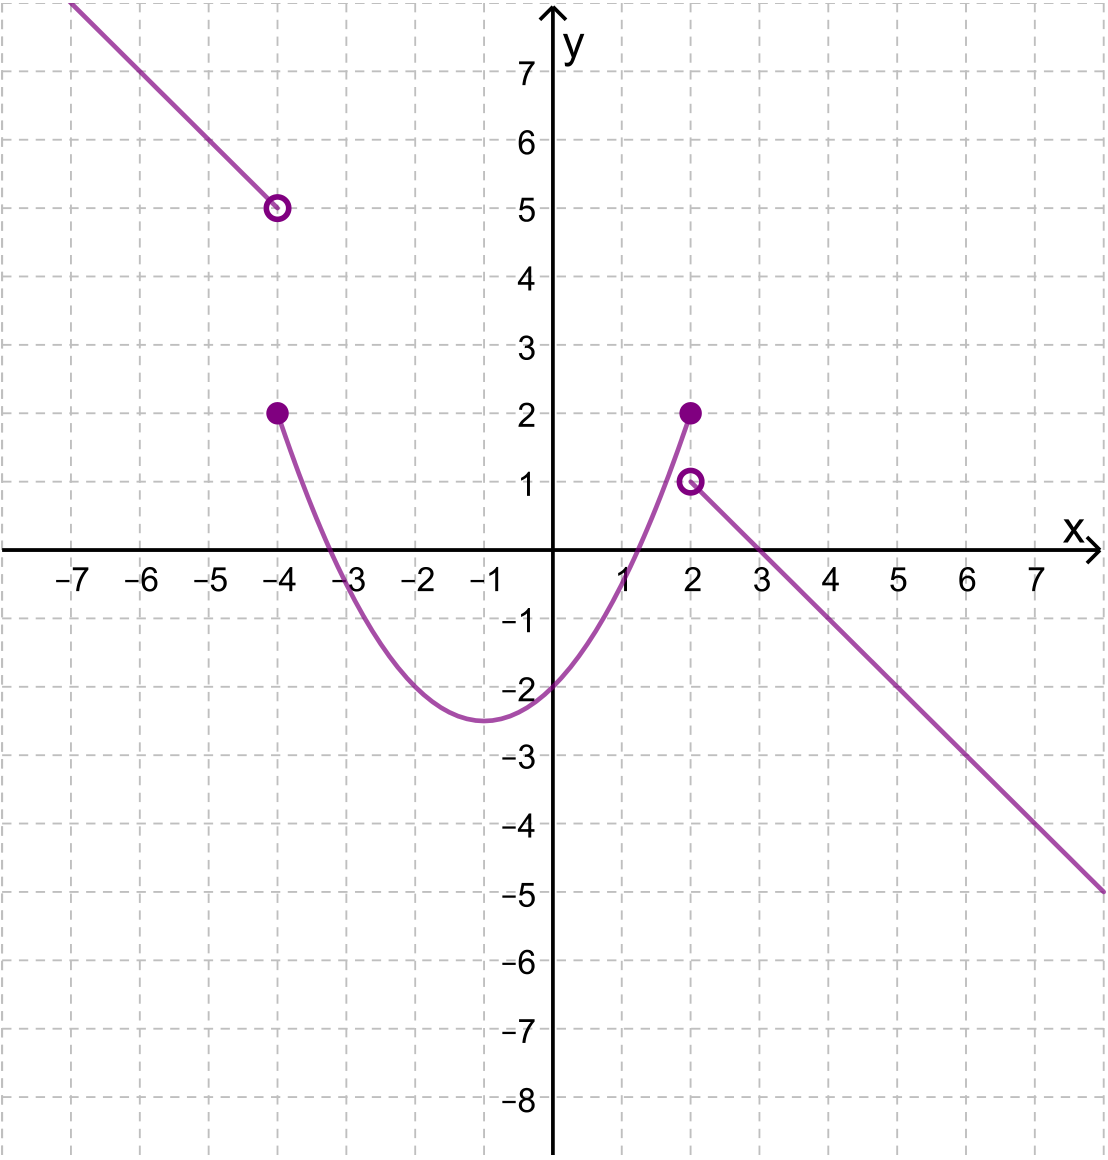
\includegraphics[width=0.5\linewidth]{3.png}
\end{figure}
\subsection*{Problem 8}
\begin{enumerate}
    \item[(d)] $f(x) = \begin{cases} 
          x - 1 & \text{if } x < -4 \\ 
          x - 2 & \text{if } -4 \leq x \leq 2 \\ 
          x - 3 & \text{if } x > 2 
          \end{cases}$ 
\end{enumerate}
\subsection*{Problem 9}
\(x^2\)
\subsection*{Problem 10}
\(-6\)
\section*{Solutions to the Set 2}
\subsection*{Problem 1}
\(|x-8|=4\)
\subsection*{Problem 2}
\(|x+4|=\dfrac{1}{2}\)
\subsection*{Problem 3}
\(x\)-intercepts \(= (-6,0),(7,0)\)\\
\(y\)-intercepts \(=(0,-12)\)

\end{document}
